% !TEX root = ../../I4PRJ, Grp3 - Dokumentation.tex
I dette afsnit beskrives designet af softwarepakken Smartpool.Application.Model. Modellaget består af de klasser der håndterer beregninger og verificering af data lokalt, inden data sendes fra applikationslaget til serveren. I modellaget findes også klasser der gemmer klient-applikationens tilstand i runtime.

Modellaget har til formål at adskille den førnævnte logik fra præsentations- og view-laget, for at overholde applikationslagets overordnede model-view-presenter arkitektur, samt at genbruge rutiner der anvendes af flere forskellige presenters. Klassediagrammet for applikationens modellag kan ses på figur~\ref{fig:application_model_cd}

\begin{figure}
	\centering
	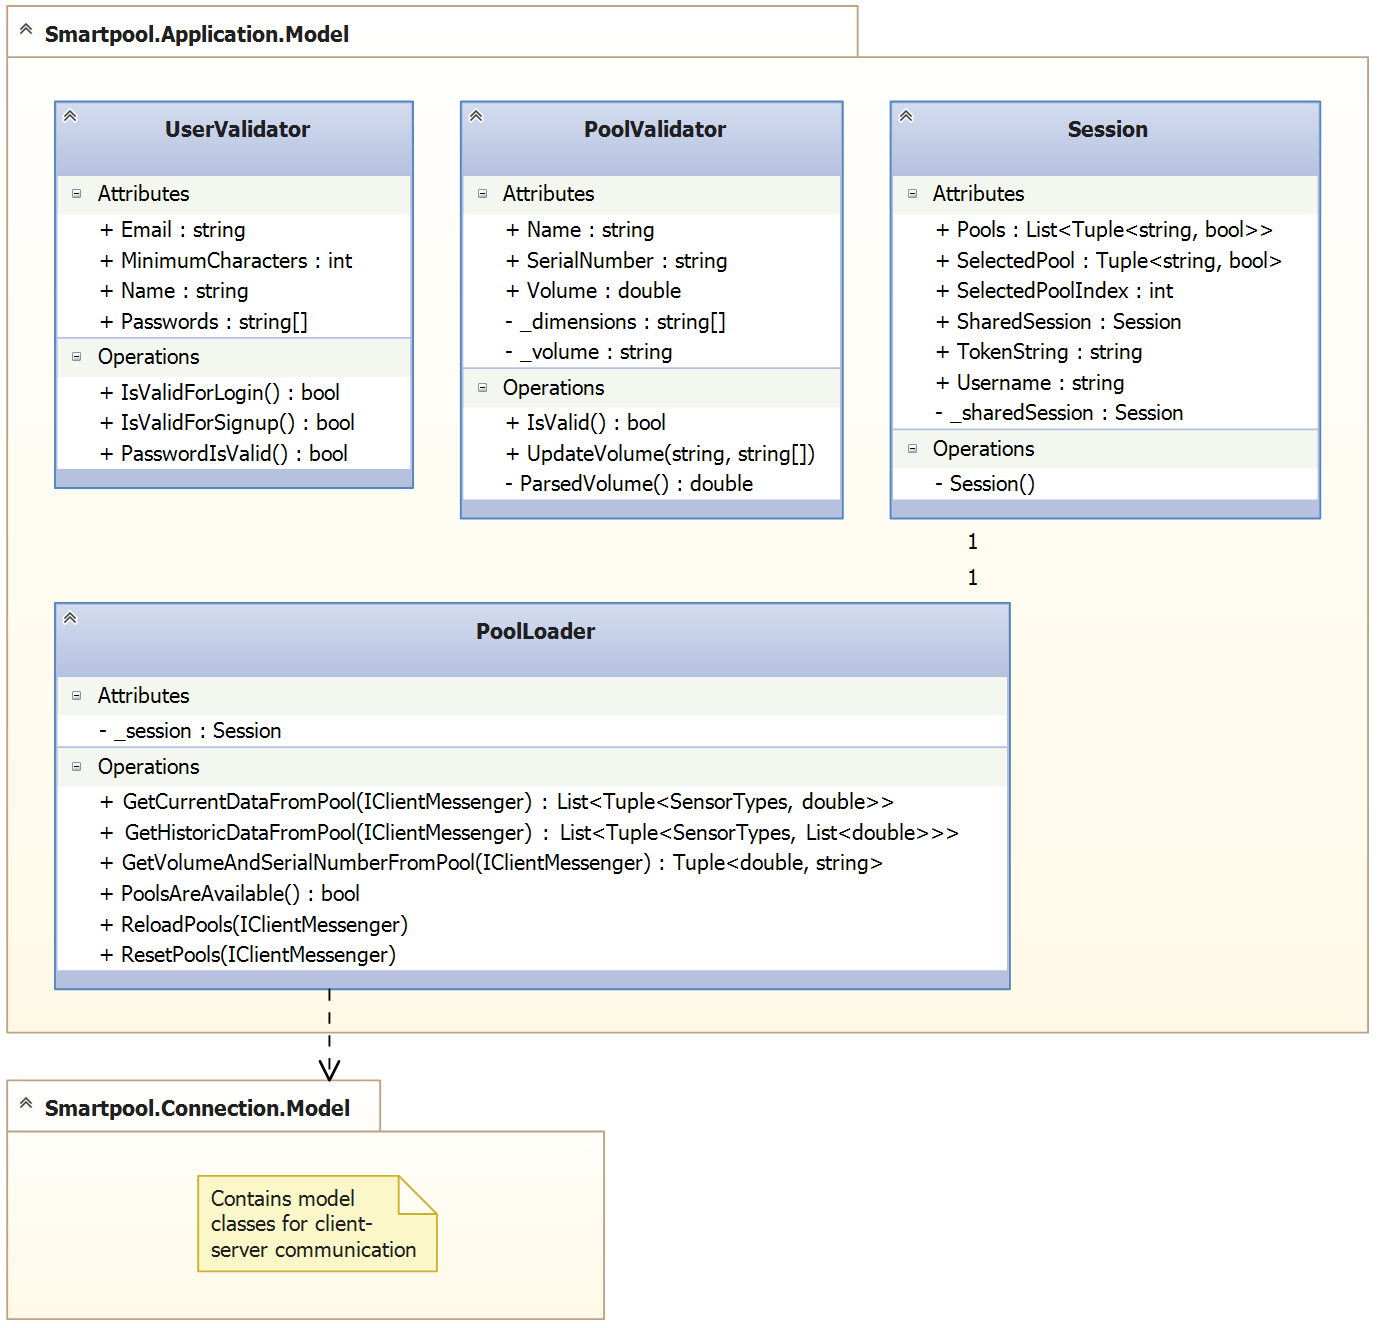
\includegraphics[width=1.0\linewidth]{figs/design/application_model_cd}
	\caption{Applikationens modellag}
	\label{fig:application_model_cd}
\end{figure}

Af diagrammet fremgår det at denne softwarepakke består af fire klasser. Det bemærkes desuden modellen har en afhængighed til Smartpool.Connection.Model, som indeholder den yderligere forbindelsesmodel, der deles af både applikationslaget og connection-server laget. I de efterfølgende afsnit beskrives de enkelte klassers design.

\subsubsection{Session}

Session er en klasse der skal gemme applikationens tilstand i runtime. Session-klassen blev designet ud fra client-server aspektet af systemets arkitektur, således at sessionsoplysninger fra serveren kunne lagres midlertidigt i applikationslaget. Session-klassen er designet som en singleton, således at applikationens tilstand kan persistere mellem overgange til forskellige views og presenters.

I Session-klassen gemmes information modtaget fra serveren (Username og TokenString) efter en forbindelse er blevet oprettet. Derudover gemmes information om hvilken pool brugeren har valgt at interagere med. En beskrivelse af Session-klassens medlemmer fremgår af tabel~\ref{tab:table_design_session}

\begin{table}
	\centering
	\begin{tabular}{| l | p{0.7\linewidth} |}
		\toprule
		\textbf{Klassemedlem}	& \textbf{Beskrivelse} \\
		\midrule
		+ Pools		& En liste med pools. En pool repræsenteres med navn og notifikationsstatus.		\\\hline
		+ SelectedPool			& En property som returnerer den pool som brugeren sidst har valgt at undersøge.	\\\hline
		+ SelectedPoolIndex				& En integer der tilsvarer den valgte pools index i listen af pools.				\\\hline
		+ SharedSession				& En property der returnere den statiske instans af Session-klassen, eller konstruere den hvis den ikke allerede findes, som følge af Singleton princippet. \\\hline
		+ TokenString					& En string indeholdende et token der bruges til kontakt med serveren. \\\hline
		+ Username						& En string indeholdende det brugernavn som brugeren af applikationen er logget ind med. \\\hline
		- sharedSession					& Backing variablen til den statiske Singleton Session. \\\hline
		- Session()							& Session-klassens constructor. Den er gjort privat for at sikre Singleton-metoden. \\
		\bottomrule
		\end{tabular}
	\caption{Beskrivelse af Session-klassens medlemmer}
	\label{tab:table_design_session}	
\end{table}

\subsubsection{PoolLoader}
PoolLoader er en klasse der har til ansvar at indkapsle den logik der omfatter indlæsning og overføring af pool-data fra client-server forbindelsen, til Session-klassen i applikationslaget. 

PoolLoader-klassen indeholder en række metoder der gør det nemmere for klasser i præsentationslaget at udføre førnævnte opgaver, således at præsentationsklasserne der indlæser pool-oplysninger kan fralægge sig dele af dette ansvar, og fokusere på præsentationslogik.

\begin{table}
	\centering
	\begin{tabular}{| l | p{0.5\linewidth} |}
		\toprule
		\textbf{Klassemedlem}	& \textbf{Beskrivelse} \\
		\midrule
		- session					& En reference til Singleton-instansen i Session-klassen, som skal bruges til lagring af information om brugerens session. \\\hline
		+ GetCurrentDataFromPool(...)	& En metode der returnere øjebliksdata fra den aktive pool i Session-instansen.	\\\hline
		+ GetHistoricDataFromPool(...) 	& En metode der returnere historisk data fra den aktive pool i Session-instansen. \\\hline
		+ GetVolumeAndSerialNumberFromPool(...)	& En metode der returnere volumen og serienummer på aktive pool i Session-instansen. \\\hline
		+ PoolsAreAvailable() 					& En metode der returnere en boolean værdi, som angiver hvorvidt Pools-listen i klassens Session-instans indeholder pools. \\\hline
		+ ReloadPools(...)						& Metoder til at indlæse eller genindlæse listen af pools på brugerens konto. \\
		+ ResetPools(...)						&  \\
		\bottomrule
		\end{tabular}
	\caption{Beskrivelse af PoolLoader-klassens medlemmer}
	\label{tab:table_design_poolloader}	
\end{table}

Mange af metoderne i PoolLoader-klassen tager imod en IClientMessenger. Denne klasse anvendes primært som interface til klienten i applikationslaget. Med interfacet kan beskeder sendes til serveren. Det er nødvendigt da PoolLoader-klassen sørger for at sende de forskellige pool-data beskeder til serveren, som kræves for at indhente den fornødne data.

\subsubsection{PoolValidator}
PoolValidator er en klasse der indkapsler valideringslogik for klasser i præsentationslaget, der enten har med oprettelse eller modificering af pools at gøre.

Klassen indeholder de properties som en almindelig pool også indeholder, samt metoder der kan kaldes for at undersøge om klassens properties er sat korrekt, i forhold til det der forventes af en pool i systemet.

\begin{table}
	\centering
	\begin{tabular}{| l | p{0.7\linewidth} |}
		\toprule
		\textbf{Klassemedlem}	& \textbf{Beskrivelse} \\
		\midrule
		+ Name				& Tekststrenge der bør sættes i forbindelse med validering af en ny pool.	\\
		+ SerialNumber			& 	\\\hline
		+ Volume 				& En property der returnere en double-repræsentation af den private volume tekststreng. \\\hline
		- dimensions 			& Private klassemedlemmer der kan indeholde oplysninger om poolens størrelse og volumen. \\
		- volume 				& 	\\\hline
		+ IsValid()					& En metode der returnere en boolean værdi, som angiver hvorvidt klassens state tillader dannelse af en ny pool. \\\hline
		+ UpdateVolume(...)						& En metode der tager imod størrelse og volumen, og opdatere de private klassemedlemmer volume og dimensions. \\\hline
		- ParsedVolume					& En metode der omdanner de to private klassemedlemmer volume og dimensions, til en double værdi. \\
		\bottomrule
		\end{tabular}
	\caption{Beskrivelse af PoolValidator-klassens medlemmer}
	\label{tab:table_design_poolvalidator}	
\end{table}

\subsubsection{UserValidator}
UserValidator er en klasse der håndterer validering af brugeroprettelse og redigering på applikationslaget, inden en forespørgsel af denne type sendes til serveren.

Klassen hjælper med at isolere brugervalideringslogik, fra klasser i præsentationslaget som håndterer brugerredigering, samt at give præsentationslaget mulighed for at sende feedback opdateringer til view-laget. Dette er også med til at aflaste serveren, da en forespørgsel med ufuldendte oplysninger ikke kan sendes til validering på serveren, mens UserValidator-klassen benyttes.

\begin{table}
	\centering
	\begin{tabular}{| l | p{0.7\linewidth} |}
		\toprule
		\textbf{Klassemedlem}	& \textbf{Beskrivelse} \\
		\midrule
		+ Name				& Tekststrenge der bør sættes i forbindelse med validering af en ny bruger.	\\
		+ Email 			& 	\\\hline
		+ MinimumCharacters  				& En integer der angiver det mindst mulige antal af karaktere der kan indgå i brugerens password. MinimumCharacters er const og kan derfor kun læses udefra. MinimumCharacters bruges af PasswordIsValid metoden til at vurdere hvorvidt et password er gyldigt. \\\hline
		+ Passwords  			& En array af tekststrenge der bruges til at gemme de passwords som indtastes af brugeren. Et array af passwords er nødvendigt da to passwords skal sammenlignes for at sikre at brugeren har indtastet passwordet rigtigt gentagende gange.\\\hline
		+ IsValidForLogin() 				& En metode der returnere en boolean værdi, som angiver hvorvidt UserValidator-klassens state tillader login. I denne metode tjekkes medlemsvariablerne Name og Passwords. \\\hline
		+ IsValidForSignup() 			& En metode der returnere en boolean værdi, som angiver hvorvidt UserValidator-klassens state tillader brugeroprettelse. I denne metode tjekkes alle medlemsvariablerne.
 \\\hline
		+ PasswordIsValid()				& En metode der sammenligner de passwords som er gemt i medlemsvariablen Passwords, og returnere en boolean der angiver hvorvidt de er ens. \\
		\bottomrule
		\end{tabular}
	\caption{Beskrivelse af UserValidator-klassens medlemmer}
	\label{tab:table_design_uservalidator}	
\end{table}